%! Author = thomas del moro
%! Date = 31/10/2023

\documentclass{article}

% Language setting
% Replace `english' with e.g. `spanish' to change the document language
\usepackage[italian]{babel}

% Set page size and margins
% Replace `letterpaper' with `a4paper' for UK/EU standard size
\usepackage[letterpaper,top=2cm,bottom=2cm,left=3cm,right=3cm,marginparwidth=1.75cm]{geometry}

% Useful packages
\usepackage{amsmath}
\usepackage{amsfonts}
\usepackage{graphicx}
\usepackage{mathrsfs}
\usepackage[colorlinks=true, allcolors=blue]{hyperref}
\usepackage{subcaption}
\usepackage{float}
\usepackage{wrapfig}

\usepackage[font=small,labelfont=bf]{caption}

\title{}
\author{Thomas Del Moro}

\begin{document}
    \maketitle
    \begin{abstract}
        Questo studio esplora l'applicazione di vari modelli di epidemie nell'ambito della fisica statistica e dei
        sistemi complessi, in particolare per quanto riguarda la dissusione di malattie infettive in una popolazione o
        la percolazione di informazioni in una rete sociale.
        Attraverso l'applicazione di questi modelli, esaminiamo fattori come la densità di popolazione, i contatti fra
        gli individui e le strategie di mitigazione basate sulla percezione del rischio.
        Le simulazioni illustrano come tali modelli possano fornire una prospettiva efficace per comprendere e gestire
        fenomeni epidemici complessi.
    \end{abstract}


    \section{Introduzione}
    La modellazione delle epidemie è un'importante area di ricerca che utilizza concetti della fisica statistica e dei
    sistemi complessi per comprendere e prevedere la diffusione delle malattie infettive.
    I modelli epidemiologici forniscono un quadro teorico per analizzare come le malattie si diffondono all'interno di
    una popolazione e come le strategie di controllo possono influenzare questa diffusione.
    Tra i modelli più conosciuti vi è il modello SIR (Susceptible-Infectious-Recovered), che suddivide la popolazione
    in tre compartimenti: suscettibili, infetti e guariti.\\
    Questi modelli, tuttavia, spesso non tengono conto della complessità delle interazioni sociali e della struttura di
    rete all'interno delle popolazioni umane.
    È però possibile, utilizzando metodi ispirati alla fisica, come la teoria
    dei grafi e la dinamica dei sistemi fuori dall'equilibrio, sviluppare modelli più sofisticati che catturino meglio
    la natura intricata delle interazioni umane.\\
    In questa revisione, esploreremo l'applicazione di vari modelli di epidemie e, attraverso simulazioni computerizzate,
    esamineremo come questi modelli possano essere utilizzati per comprendere e gestire fenomeni epidemici complessi.


    \section{Forest Fire}
    Il modello più semplice di un'epidemia trascura completamente la dinamica dell'agente virale. Se supponiamo inoltre
    che gli ospiti non si muovano e siano disposti su una griglia regolare con una certa densità.
    Otteniamo in questo modo il modello di diffusione di un incendio boschivo senza vento (Forest Fire).\\
    Ogni cella della griglia può essere in uno di tre stati: vuota, occupata da un albero sano o occupata da un albero
    incendiato. Per semplicità abbiamo trascurato il caso di albero già bruciato (immune), che vedremo nella prossima sezione.\\
    Il processo di diffusione segue una curva a S, più o meno ripida e lunga a seconda del parametro di densità.
    In particolare, se la densità è troppo bassa, l'incendio si estinguerà rapidamente, mentre se questa è alta l'incendio
    di propagherà a tutto il reticolo.
    \begin{figure}[H]
        \centering
        \begin{subfigure}[b]{0.49\linewidth}
         \centering
         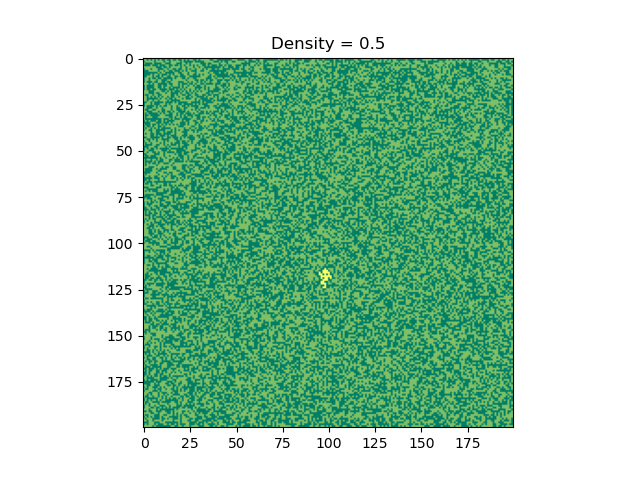
\includegraphics[width=\linewidth]{../images/forestfire_single05image}
     \end{subfigure}
        \hfill
        \begin{subfigure}[b]{0.49\linewidth}
         \centering
         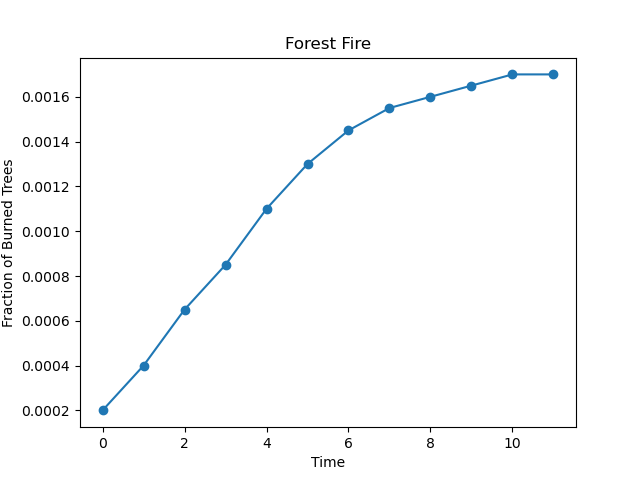
\includegraphics[width=\linewidth]{../images/forestfire_single05}
     \end{subfigure}
     \hfill
     \begin{subfigure}[b]{0.49\linewidth}
         \centering
         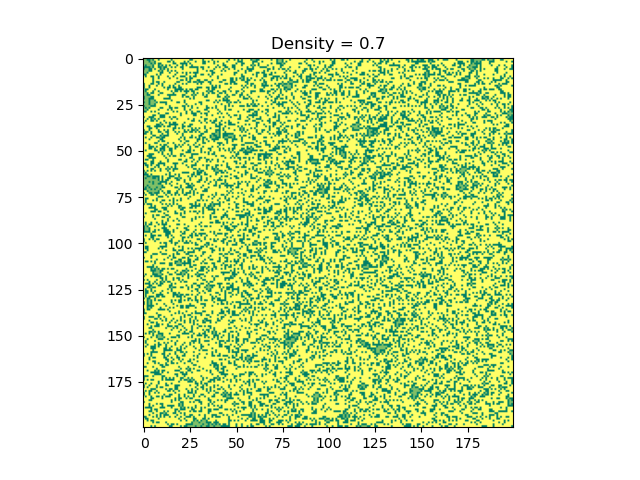
\includegraphics[width=\linewidth]{../images/forestfire_single07image}
     \end{subfigure}
        \hfill
        \begin{subfigure}[b]{0.49\linewidth}
         \centering
         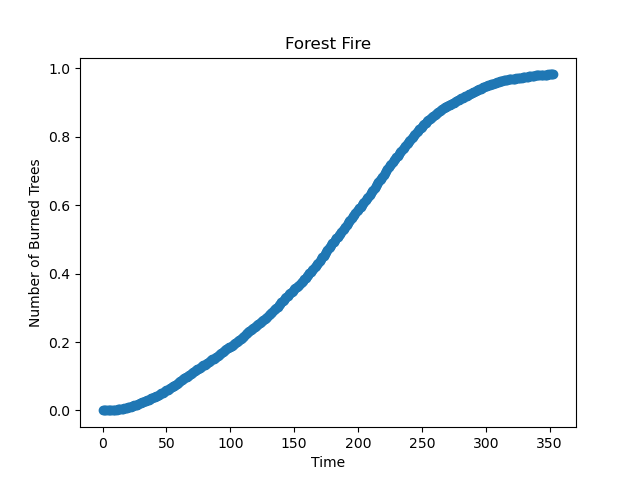
\includegraphics[width=\linewidth]{../images/forestfire_single07}
     \end{subfigure}
     \caption{Simulazioni del modello Forest Fire con densità 0.5 (in alto) e 0.7 (in basso). Sulla sinistra si possono
     osservare le immagini del reticolo, mentre sulla destra la curva di diffusione dell'incendio.}
     \label{fig:forestfire}
    \end{figure}
    Notiamo facilmente che se la densità è relativamente bassa, è probabile che l'incendio di estingua velocemente.
    Possiamo quindi osservare il numero finale di alberi incendiati al variare della densità del reticolo. I risultati,
    mostrati nel grafico in Figura \ref{fig:forestfire_density}, evidenziano di nuovo una curva a S, con un punto di
    transizione tra un regime in cui l'incendio si estingue rapidamente e uno in cui si propaga a tutto il reticolo.
    \begin{figure}[H]
        \centering
        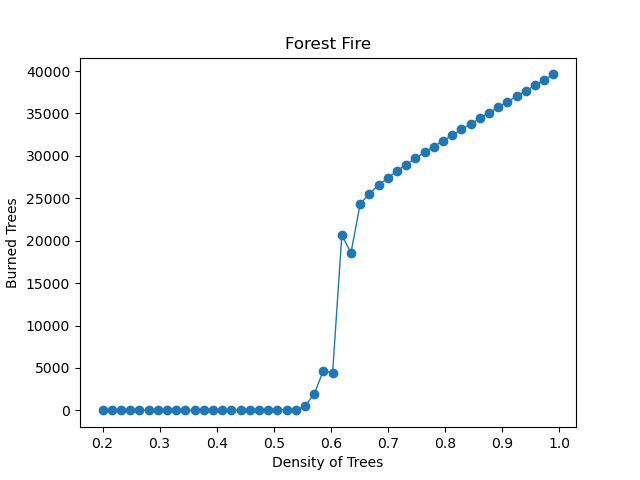
\includegraphics[width=0.6\linewidth]{../images/forestfire_final}
        \caption{Numero finale di alberi incendiati al variare della densità del reticolo.}
        \label{fig:forestfire_density}
    \end{figure}



    \section{SIR}
    Il modello SIR rappresenta uno dei più conosciuti e più semplici modelli epidemiologici.
    È in parte analogo al modello Forest Fire, ma con una dinamica probabilistica, leggermente più complessa di quella vista sopra.\\
    Supponiamo di avere una popolazione di $N$ individui disposti su una griglia. In questo caso tutte le celle sono
    occupate da un individuo, ma questo, ad ogni istante di tempo, sarà infettato dagli individui vicini solo con una certa probabilità $p$.
    Le celle possono dunque essere suddivise nelle tre categorie:
    \begin{itemize}
        \item \textbf{Suscettibili (S)}: individui sani che possono essere infettati.
        \item \textbf{Infetti (I)}: individui infetti che possono infettare gli individui sani.
        \item \textbf{Refrattari (R)}: individui infettati e guariti che non possono più ammalarsi (immuni).
    \end{itemize}
    Per eseguire le simulazioni possiamo inizializzare il reticolo con un numero arbitrario di infetti e osservare come la malattia si diffonde a
    seconda dei parametri di infettività e di guarigione, fino a che non sarà più in grado di infettare nuovi individui.
    \begin{figure}[H]
        \centering
        \begin{subfigure}[b]{0.49\linewidth}
         \centering
         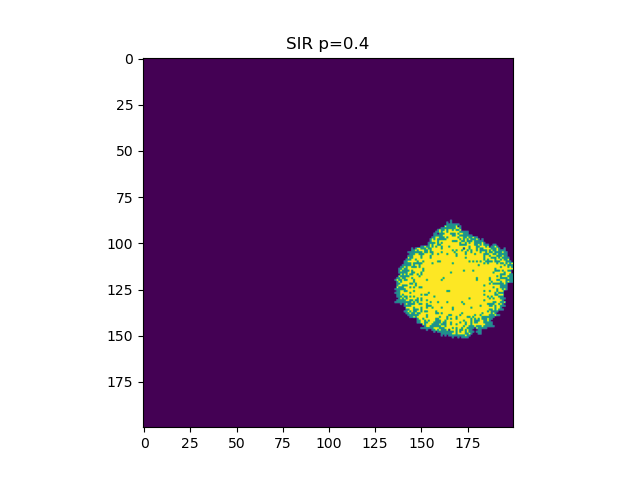
\includegraphics[width=\linewidth]{../images/sir_image1}
     \end{subfigure}
        \hfill
        \begin{subfigure}[b]{0.49\linewidth}
         \centering
         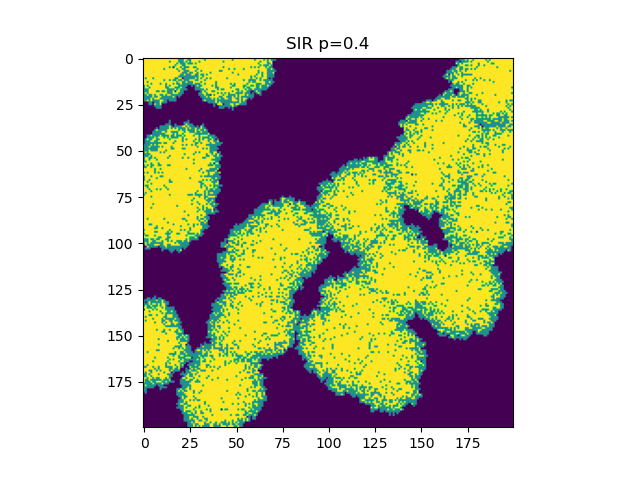
\includegraphics[width=\linewidth]{../images/sir_image20}
     \end{subfigure}
     \caption{Simulazioni del modello SIR rispettivamente a partire da 1 infetto (sinistra) e da 20 infetti (destra).}
     \label{fig:sir_image}
    \end{figure}
    Le curve caratteristiche del modello SIR possono essere ottenute applicando le assunzioni di campo medio, ovvero
    eliminando le correlazioni spaziali tra gli individui. In questa relazione ci limiteremo a confrontare le curve teoriche
    con quelle empiriche ottenute dalle simulazioni sopra descritte. Tale indagine è mostrata in Figura \ref{fig:sir_curves}.
    \begin{figure}[H]
        \centering
        \begin{subfigure}[b]{0.49\linewidth}
         \centering
         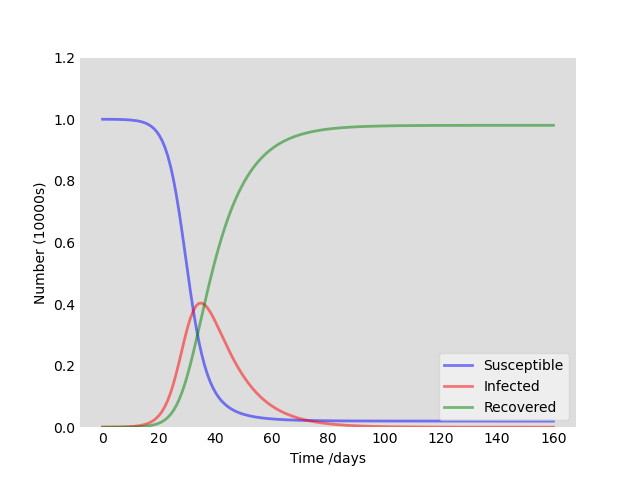
\includegraphics[width=\linewidth]{../images/sir_equations}
            \caption{Curve teoriche del modello SIR}
        \end{subfigure}
        \hfill
        \begin{subfigure}[b]{0.49\linewidth}
         \centering
         \includegraphics[width=\linewidth]{../images/sir_curves1}
            \caption{Curve empiriche di una simulazione del modello SIR}
        \end{subfigure}
        \caption{Curve caratteristiche teoriche ed empiriche del modello SIR.}
        \label{fig:sir_curves}
    \end{figure}

    Il fattore più critico per la diffusione della malattia è la probabilità di infezione $p$. Nel modello molto semplice
    abbiamo realizzato, l'infezione si diffonde molto probabilmente in tutto il reticolo anche con un livello di infettività
    relativamente basso: Ciò che possiamo osservare è quindi una diversa velocità di propagazione dell'epidemia a seconda
    di questo parametro.
    \begin{figure}[H]
        \centering
        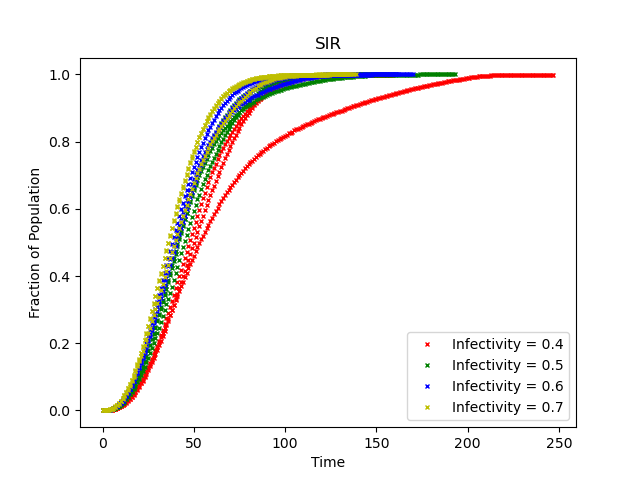
\includegraphics[width=0.6\linewidth]{../images/sir_infectivities}
        \caption{Curve di diffusione di più simulazioni al variare della probabilità di infezione.}
        \label{fig:sir_infectivities}
    \end{figure}
    Possiamo notare in Figura \ref{fig:sir_infectivities} che all'aumentare della probabilità di infezione, la curva di
    individui refrattari, ovvero infettati e guariti, si sposta verso sinistra, indicando una maggiore velocità di
    propagazione dell'epidemia.\\
    Un ulteriore fattore critico oltre ai due già descritti è dato dal numero di vicini scelti per ogni individuo. In una tale griglia
    è possibile scegliere di considerare solo i primi 4 vicini (alto, basso, destra, sinistra) oppure tutte le 8 celle adiacenti.
    In questo ultimo caso ci aspettiamo che la soglia di infettività sia più bassa, in quanto la probabilità di trovarsi
    vicino a un individuo suscettibile è maggiore. Possiamo infatti notare in Figura \ref{fig:sir_neighbors} che la curva
    relativa agli 8 vicini è più ripida rispetto a quella relativa agli 4 vicini.
    \begin{figure}[H]
        \centering
        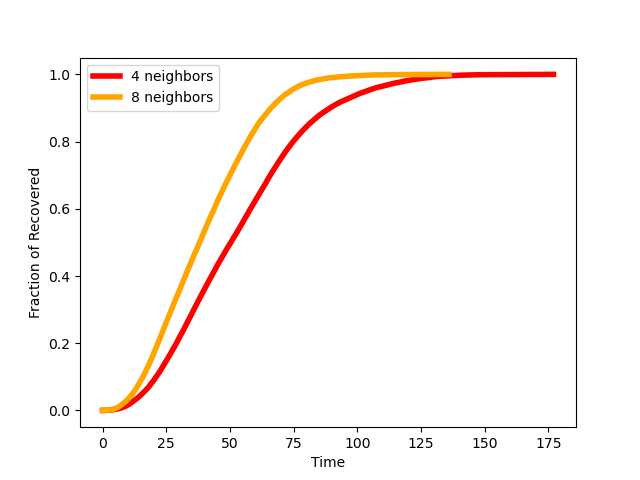
\includegraphics[width=0.6\linewidth]{../images/sir_neighbors}
        \caption{Frazione di individui refrattari relativi a una simulazione con $p=0.8$}
        \label{fig:sir_neighbors}
    \end{figure}

    Questo modello molto semplice non tiene ovviamente conto di caratteristiche molto più complesse della malattia e della
    popolazione, come la mobilità degli individui, la densità di popolazione, la distribuzione dell'età e la presenza di
    misure di mitigazione come il distanziamento sociale e la quarantena. Tuttavia, fornisce una base teorica per
    comprendere la diffusione delle malattie infettive e come le strategie di controllo possono influenzare questa diffusione.

    \section{SIS}
    Il modello SIR assume che gli individui guariti acquisiscano immunità permanente alla malattia.
    Tuttavia, se ciò non valesse, esistono modelli alternativi che considerano una certa probabilità di reinfezione.
    Il caso all'estremo opposto è infatti il modello SIS (Susceptible-Infectious-Susceptible), in cui gli individui
    guariti tornano a essere suscettibili in egual maniera rispetto ai sani.
    Questo modello è particolarmente interessante per le malattie in cui l'immunità non è permanente, come l'influenza
    stagionale o il raffreddore comune.\\
    Anche per questo modello possiamo eseguire delle simulazioni analoghe alle precedenti, utilizzando lo stesso reticolo ma
    assumendo che gli individui guariti tornino a essere suscettibili.
    \begin{figure}[H]
        \centering
        \begin{subfigure}[b]{0.49\linewidth}
         \centering
         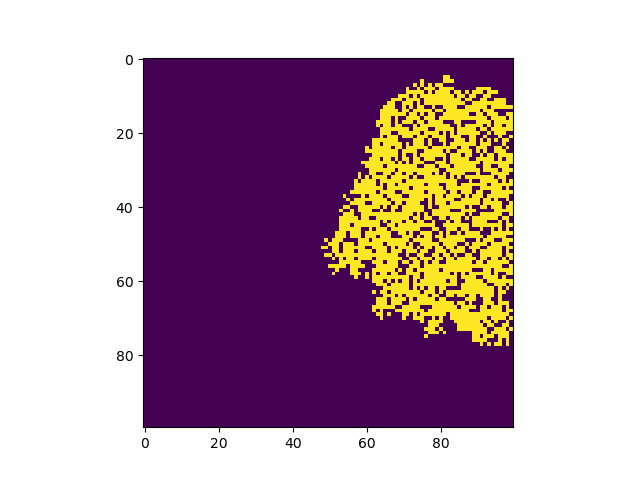
\includegraphics[width=\linewidth]{../images/sis_image1}
     \end{subfigure}
        \hfill
        \begin{subfigure}[b]{0.49\linewidth}
         \centering
         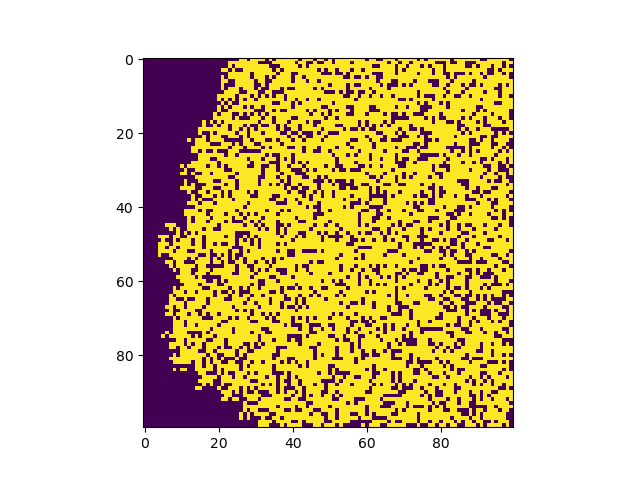
\includegraphics[width=\linewidth]{../images/sis_image2}
     \end{subfigure}
     \caption{Simulazione del modello SIS con infettività $p=0.2$ e tasso di guarigione $r=0.5$.}
     \label{fig:sis_image}
    \end{figure}
    In questo caso le curve saranno diverse da quelle del modello SIR, poiché non abbiamo una frazione di refrattari.
    A seconda del grado di infettività e di guarigione è possibile osservare andamenti diversi tra loro, ma che hanno
    tutti la caratteristica che avere un andamento asintotico nel lungo termine simile a una saturazione. In Figura
    \ref{fig:sis_curves} sono mostrati i risultati ottenuti con diversi valori dei parametri di infettività e di guarigione.
    \begin{figure}[H]
        \centering
        \begin{subfigure}[b]{0.49\linewidth}
         \centering
         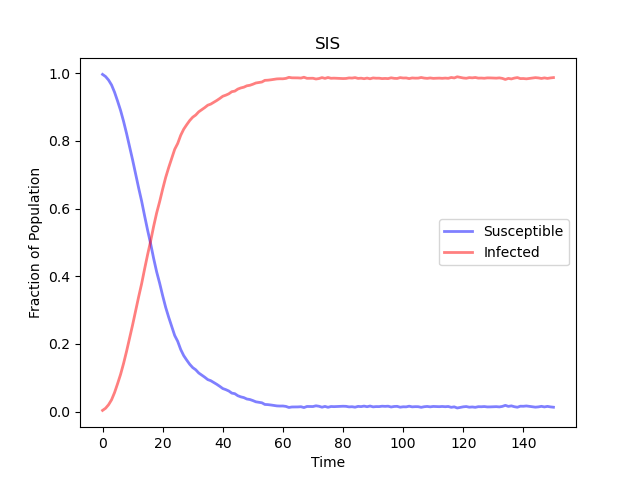
\includegraphics[width=\linewidth]{../images/SIS_curves}
            \caption{Simulazione SIS con $p=0.6$ e $r=0.2$}
     \end{subfigure}
        \hfill
        \begin{subfigure}[b]{0.49\linewidth}
         \centering
         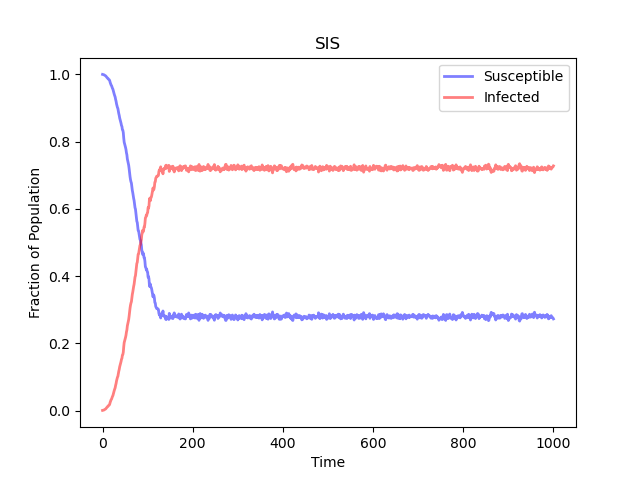
\includegraphics[width=\linewidth]{../images/SIS_curves1}
            \caption{Simulazione SIS con $p=0.2$ e $r=0.5$}
     \end{subfigure}
     \caption{Curve empiriche di due simulazioni del modello SIS.}
     \label{fig:sis_curves}
    \end{figure}

    \section{Percolazione}


    \section{Conclusioni}

    \begin{thebibliography}{9}
\bibitem{lapucci}
Matteo Lapucci, Davide Pucci (2023) \emph{Mixed-integer quadratic programming reformulations of multi-task learning models}

\bibitem{c-kmeans}
P. S. Bradley, K. P. Bennett, A. Demiriz (2000) \emph{Constrained K-Means Clustering}

\bibitem{b-kmeans}
Mikko I. Malinen, Pasi Fränti (2014) \emph{Balanced K-Means for Clustering}

\end{thebibliography}

\end{document}
